\newpage
\section{Urto}
Un \textbf{urto} tra punti materiali / corpi rigidi avviene in un intervallo temporale 
$t_0 - \epsilon < t < t_0 + \epsilon$ molto breve, rispetto alla dinamica del sistema.\\\\
Le reazioni vincolari sono difficili da descrivere con precisione. Ci interessa invece lo stato del sistema \textbf{subito prima}
($t_0^- \equiv t_0 - \epsilon$) e \textbf{subito dopo} ($t_0^+ = t_0 \epsilon$). 
Durante l'urto le forze che non sono generate dal contatto sono spesso di intensità trascurabile.
\begin{definition}
    Definisco \textbf{vetore impulso di una forza} $\vec{F}(t)$ un intervallo temporale $[t_0 - \epsilon, t_0 + \epsilon]$
    $$\vec{I}_{\epsilon} = \int_{t_0 - \epsilon}^{t_0 + \epsilon}dt \cdot \vec{F}(t) \hspace{10pt} \text{e} \hspace{10pt}\vec{I} = \lim_{\epsilon\to 0}\vec{I}_{\epsilon}$$
\end{definition}
\hspace{-15pt}Dico che $\vec{F}(t)$ è una \textbf{forza impulsiva} se $||\vec{I}|| \neq 0$ altrimenti la forza è non impulsiva.
Una forza la cui intensità è limitata non può essere impuliva.\\\\
Le coordinate sono funzioni continue del tempo (non ci può essere "teletrasposrto"), ess. $\vec{r}(t_0^+) = \vec{r}(t_0^-)$ mentre
velocità, accelerazione, quantità di moto, momento angolare, energia cinetica possono subire variazioni tra $t_0 - \epsilon$ e $t_0 + \epsilon$.\\\\
Se l'energia cincetica \textbf{del sistema} non vaira tra $t_0 - \epsilon$ e $t_0 + \epsilon$ ("è conservata") l'urto si dice \textbf{elastico}, altrimenti \textbf{anelastico}.
Se dopo l'urto si viene a formare un corpo rigido, l'urto è \textbf{completamente anelastico}.
\begin{figure}[h!]
    \centering
    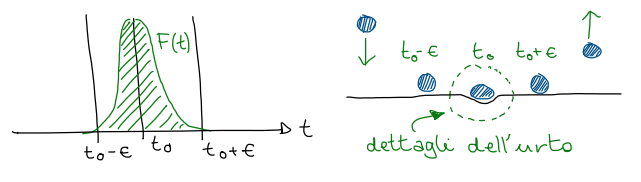
\includegraphics[width=0.65\textwidth]{images/vettore-impulso-forze.png}
\end{figure}

\subsection{Equazioni cardinali e teorema forze vive in forma impulsiva}
Integro entrabi i membri da $t_0 - \epsilon$ a $t_0 + \epsilon$
$$I. \:\:\: m\ddot{\vec{r}}_{CM}(t) = \sum_i \vec{F}_i^{(E)}(t) \Rightarrow m\dot{\vec{r}}_{CM}(t_0^+) - m\dot{\vec{r}}_{CM}(t_0^-) = \sum_i \vec{I}_i^{(E)}$$
$\vec{I}_i^{(E)}$ vuol dire che sono le $\vec{F}_i$ impulsive contano.
$$II. \:\:\: \dot{\vec{L}}_p(t) = \sum_i(\vec{r}_i(t) - \vec{r}_p(t)) \times \vec{F}_i^{(E)} - \dot{\vec{r}}_p(t) \times M\dot{\vec{r}}_{CM}(t) \Rightarrow \vec{L}_p(t_0^+) - \vec{L}_p(t_0^-) = \sum_i(\vec{r}_i(t_0) - \vec{r}_p(t_0)) \times \vec{I}_i(E)$$
Anche in questo caso sole le $\vec{F}_i$ impulsive contano, in oltre come si nota in $M\dot{\vec{r}}_{CM}(t)$ le velocità rimangono limitate.
\begin{example}
    Non ci sono forze esterne impulsive.
    \begin{figure}[h!]
        \centering
        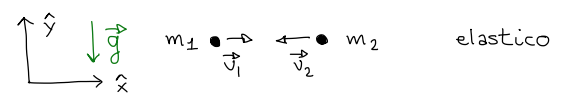
\includegraphics[width=0.6\textwidth]{images/ess-elastico.png}
    \end{figure}
    $$m_i\dot{x}_i(t_0^+) + m_2\dot{x}_2(t_0^+) - m_1\dot{x}_1(t_0^-) - m_2\dot{x}_2(t_0^-) = 0$$
    Notiamo che $\dot{x}_1(t_0^-) = v_1$ e $ m_2\dot{x}_2(t_0^-) = v_2$. L'urto è elastico
    $$\frac{1}{2}m_1\dot{x}_1(t_0^+)^2 + \frac{1}{2}m_2\dot{x}_2(t_0^+)^2 - \frac{1}{2}m_1\dot{x}_1(t_0^-)^2 - \frac{1}{2}m_2\dot{x}_2(t_0^-)^2 = 0$$
    $$\Rightarrow \dot{x}_2 (t_0^+) = v_2 - \frac{m_1}{m_2}[\dot{x}_1 (t_0^+) - v_1] \Rightarrow \frac{1}{2}m_1\dot{x_1}(t_0^+)^2 + \frac{1}{2}m_2 \{v_2 - \frac{m_1}{m_2}[\dot{x_1}(t_0^+) - v_1]\}^2$$
    $$-\frac{1}{2}m_1 v_1^2 - \frac{1}{2}m_2v_2^2 = 0$$
    $$\dot{x}_1(t_0^+) = \frac{m_1 - m_2}{m_1 + m_2}v_1 + \frac{2m_2}{m_1+m_2}v_2$$
\end{example}
\begin{example}
    Piano liscio, urto elastico. Liscio: la relazione vincolare impulsiva è solo normale.
    \begin{figure}[h!]
        \centering
        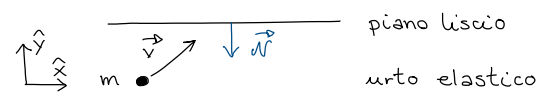
\includegraphics[width=0.6\textwidth]{images/ess-piano-liscio-urto-elastico.png}
    \end{figure}
    $$\begin{cases}
        m\dot{x}(t_0^+) - m\dot{x}(t_0^-) = 0\\
        m\dot{y}(t_0^+) - m\dot{y}(t_0^-) = N \text{ impulso relazione vincolare}
    \end{cases}$$
    $$\frac{1}{2}m[\dot{x}(t_0^+)^2 + \dot{y}(t_0^+)^2] - \frac{1}{2}m[\dot{x}(t_0^-)^2 + \dot{y}(t_0^-)^2] = 0 \Rightarrow \dot{x}(t_0^+) = \dot{x}(t_0^-) \text{ non cambia }$$
    $$\dot{y}(t_0^+)^2 - \dot{y}(t_0^-)^2 = 0 \Rightarrow \dot{y}(t_0^+) - \dot{y}(t_0^-) \text{ si inverte } \Rightarrow N = 2m\dot{y}(t_0^-)$$
\end{example}
\begin{example}
    Minimo $\mu_s$ per un "wallrun"?
    \begin{figure}[h!]
        \centering
        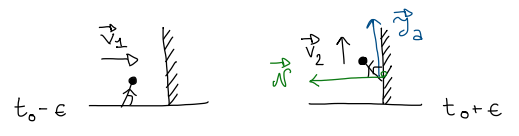
\includegraphics[width=0.6\textwidth]{images/ess-wallrun.png}
    \end{figure}
    $$\dot{\vec{r}}(t_0^-) = v_1 \hat{x} \hspace{15pt} \dot{\vec{r}}(t_0^+) = v_2\hat{y}$$
    $$
    \begin{cases}
        m\dot{x}(t_0^+) - m\dot{x}(t_0^-) = -N\\
        m\dot{y}(t_0^+) - m\dot{y}(t_0^-) = I_a
    \end{cases}
    \Rightarrow
    \begin{cases}
        N = mv_1 \\
        I_a = mv_2
    \end{cases}
    $$
    Da $||\vec{F}_a|| \leq \mu_s||\vec{N}||$, integrando membro a membro, segue $I_a \leq \mu_s N \Rightarrow \mu_s \geq \frac{mv_2}{mv_1} = \frac{v_2}{v_1} = \mu_s,min$
\end{example}
\begin{example}
    Urto anelastico asta-perno. Massimo $\Theta$?
    \begin{figure}[h!]
        \centering
        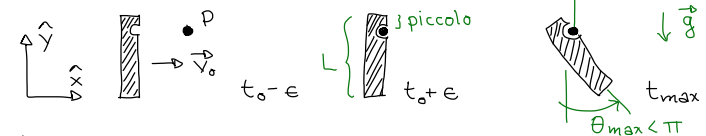
\includegraphics[width=0.6\textwidth]{images/urto-anaelastico-asta-perno.png}
    \end{figure}

    \hspace{-15pt}L'urto forza esterna impulsiva è la relazione vincolare in P, che però ha momento nullo rispetto a P.
    $$\vec{L}_p(t_0^+) - \vec{L}_p(t_0^-) = 0 \hspace{10pt}\vec{L}_p(t_0^-) = (\vec{r}_{CM}(t_0^-) - \vec{r}_p) \times M\dot{\vec{r}}_{CM}(t_0^-) = -\frac{L}{2}\hat{y} \times Mv_0 \hat{x} = \frac{1}{2}MLv_0\hat{z}$$
    Solo il momento angolare "del CM" è non nullo.
    $$\vec{L}_p(t_0^+) = \frac{1}{2}ML \frac{L}{2}\dot{\Theta}(t_0^+)\hat{z} + (\frac{1}{12}ML^2)\dot{\Theta}(t_0^+)\hat{z} = \frac{1}{3}ML^2 \dot{\Theta}(t_0^+)\hat{z}$$
    $$\frac{1}{3}ML^2\dot{\Theta}(t_0^+) - \frac{1}{2}MLv_0 = 0 \Rightarrow \dot{\Theta}(t_0^+) = \frac{3}{2}\frac{v_0}{L}$$
    Per $t > t_0$ l'energia si conserva perché le forze che fanno lavoro sono conservative. La relazione in P non è conservativa ma P è fermo e c'è attrito.
    $$\frac{1}{2}M[\frac{L}{2}\dot{\Theta}(t_0^+)]^2 + \frac{1}{2}(\frac{1}{12}ML^2)\dot{\Theta}(t_0^+)^2 - Mg\frac{L}{2} = -Mg \frac{L}{2}\cos\Theta_{max}$$
    $$\Rightarrow Mg \frac{L}{2}(1 - \cos\Theta_{max}) = \frac{1}{1}\cdot \frac{1}{3}ML^2\dot{\Theta}(t_0^+)^2 = \frac{1}{6}ML^2 \frac{g}{4} - \frac{v_0^2}{L^2} \Rightarrow 1 - \cos\Theta_{max} = \frac{3}{4}\frac{v_0^2}{gL} \hspace{10pt}\Theta_{max} = \arccos(1-\frac{3}{4}\frac{v_0^2}{gL})$$
\end{example}